\documentclass{llncs}
%\documentclass{acm_proc_article-sp}
\usepackage[lined,boxed,commentsnumbered, ruled]{algorithm2e}
\usepackage{amssymb,amsmath}
\usepackage{epsfig,graphicx,subfigure}
\usepackage{multirow}


\begin{document}
\title{Context Aware Recommendation on Missing not at Random Contextual Texts}
%% use optional labels to link authors explicitly to addresses:
\author{Dugang Liu\inst{1} \and Chen Lin\inst{1}}
\institute{Department of Computer Science, Xiamen University \email{chenlin@xmu.edu.cn}}
\maketitle

\begin{abstract}

\end{abstract}

\section{Introduction}\label{sec:intro}
% Context Aware Recommendation: importance, 
Context Aware Recommendation System (CARS) has recently attracted  interest from both academy and industry. CARS is welcomed by enterprises and users because it delivers more accurate and reasonable recommendation by taking contextual information into account. The contextual information includes and is not limited to when, where and with whom the user is to purchase an item. CARS has been successfully applied in a bunch of areas, including travel~\cite{Biancalana2013Approach}, music~\cite{Cai2007MusicSense}, web news~\cite{Wang2015CROWN} and so on. 


%contextual information gather from text, related work survey
The input of CARS is user feedback (i.e. user-item ratings) and the corresponding contextual information. Contextual information can be gathered from various sources. The era of Web 2.0 has kindled massive growth of opinions and reviews on the web. Therefore more and more researchers explore the feasibility of building CARS based on online reviews~\cite{Li2010Contextual,Levi2012Finding,Hariri2013Query,Liu2013Combining,Marcelo2016Mining}. They adopted text mining techniques to extract contextual information from online reviews and transform a rating into a contextual rating. Then conventional recommendation models are built on contextual ratings.

%disadvantage: sparsity. (1) no context 
Generally CARS suffers from the data sparsity problem. We have to deal with two challenges related to sparse contextual user feedback. First of all, \textbf{the missing of contextual information in ratings and reviews}. Even with powerful text mining techniques, the amount of user feedback with contextual information is far from sufficient to train a promising recommendation model. Users do not always provide contextual information when they give ratings and reviews. Below we show several examples of online reviews with and without implications on the contexts.

%example here
\begin{figure}[!ht]
\label{fig:example}
\centering
\includegraphics[width=0.8\textwidth]{example.eps}
\caption{Selected reviews for two restaurants from www.yelp.ca. Reviews are shortened for the limited space. Number of starts for each indicate user rating. Reviews in violet rectangles are context explicit feedback, reviews in yellow rectangles are context implicit feedback}
\end{figure}

% problem: missing? not at random
Existing research efforts simply discard reviews without any contextual information. They fail to make full use of user feedback, because the rating could still be informative even that the context is not given. We  show here that this strategy is problematic when the contextual information in reviews are missing not at random.  For example, many social studies have found that users write online reviews to ``brag or moan''~\cite{}, therefore online users give the contextual information on purpose in respond to an extreme experience under the given contexts. Consider the illustrative example in Fig~\ref{fig:example}. On the left  the user is satisfied with ... under context ... On the right, the user is ...

%MNAR assumption
To address the above problem, we propose a novel model which is based on missing not at random assumptions. To connect the dots among ratings, non-contextual reviews and contextual reviews, we borrow the ideas of marginal utility theory~\cite{samuelson1937note}. Utility surplus is an economic concept to measure a consumer's ``satisfaction'' or ``pleasure''. Utility surplus is the difference between what a consumer pays and what a consumer gains. We expand the definition of utility surplus to a context aware setting: what a consumer benefits from a purchase under the specific context. We then assume that the user will compare the general utility surplus given no context and the context aware utility surplus under a specific context. The probability of he/she giving a contextual review is dependent on the result of the comparison.

%(2) high dimensional 
The second issue is \textbf{the high dimensionality of context space}. Most prior works modeled the ratings as a hypercube. With the massive number of possible values for each contextual dimension, the data sparsity problem is more severe. Take the location context for example, the purchase could happen at any place, thus it is very difficult to collect enough  ratings which occur in the same place. 


% model contextual scenario
A strategy that departs from data cube approach is to project contextual ratings into hidden lower dimensional contextual spaces which consist of a set of contextual scenarios. We follow this path because it can be naturally incorporated into our models. The utility is the aggregation of user preferences over several commodity features of interest.  We assume that the contextual utility is associated to a contextual scenario and the contextual information in the review texts are distributed depending on the contextual scenario.  


% contribution: first MNAR in context aware recommendation and text mining 

Our contributions are three folds. (1) To the best of our knowledge, our work is the first in literature to apply MNAR properties to CARS and text mining based recommendations.  We incorporate the utility theory in this novel model. (2) We address the data sparsity problem by exploiting non contextual reviews and embedding in a dimension reduction model. (3) We deliver recommendations that are both accurate and more explainable. 

% paper structure 

The rest of this paper is organized as follows. We provide a brief discussion on related work in section~\ref{sec:related}. We introduce the model on missing not at random contextual texts in section~\ref{sec:mnar}. We then detail the application of this model in context aware recommendation in section~\ref{sec:method}. The experimental results are described and analyzed in section~\ref{sec:exp}. Finally, we conclude our work in section~\ref{sec:con}.

\section{Related Work}\label{sec:related}
This work is related to two areas: contextual aware recommendation systems and online review mining.
\subsection{Context Aware Recommendation Systems}
%recsys
%Most recommender systems use numeric user ratings to construct a rating matrix, and apply collaborative filtering approaches to recommend items for users with similar tastes~\cite{Bobadilla2013Recommender}. There are two types of collaborative filtering techniques. One is based on retrieving nearest neighbors, performances of which are enhanced by modifying the similarity measurements, such as removing the global effect of nearest neighbors~\cite{Bell2007Scalable}. The other is based on matrix factorization~\cite{Koren2009Matrix} to approximate the observed ratings with hidden user preferences and item features. Probabilistic versions of matrix factorization are also prodominant~\cite{salakhutdinov2008probabilistic}. For binary relevance data, researchers present methodologies that target different object functions, most of which are ranking related measures. For example, BPR~\cite{Rendle2009BPR} maximizes the likelihood of pair-wise rankings, CliMF~\cite{Shi2012CLiMF} directly maximizes the mean reciprocal rank to improve top-k recommendations, ListRank-MF~\cite{Shi2010Listwise} minimizes a loss function that represents the uncertainty between training lists and output lists.
%CARS
CARS is an emerging topic in recommender community~\cite{Adomavicius2011Context}. The performance of CARS has been verified by a live controlled experiment~\cite{Gorgoglione2011Effect}. There are three types of approaches to incorporate contextual information in the recommendation process. The first type is to pre-filter, i.e. select contextualized ratings data and factorize each context specific rating matrix~\cite{Adomavicius2005Incorporating}. The second type is to post-filter, i.e. split the resulting items to different contexts after recommendation~\cite{Baltrunas2009Context}. The third type is to model the context, i.e. as a latent variable in BNN~\cite{Palmisano2008Using}, or as a latent factor in matrix factorization~\cite{Baltrunas2011Context}. or as tensor factorization~\cite{Wang2015CROWN,Karatzoglou2010Multiverse}. Empirical study has shown that which approach is better depends on the application~\cite{Panniello2009Experimental}. The sparsity of rating data is an obstacle for CARS. A typical improvement is to integrate other resources, i.e. demographic information~\cite{Li2011Towards}, sequential patterns~\cite{Hariri2012Context}, or, as we might review in the next subsection, texts in online reviews~\cite{Li2010Contextual,Levi2012Finding,Hariri2013Query,Liu2013Combining}.

\subsection{Online Review Mining}
Online review mining has been an active research area. Most existing researches are efforts that summarize reviews and extract certain information, i.e. opinion polarities~\cite{Liu2005Opinion}, user groups according to their interests~\cite{Si2014Users}, aspects of products~\cite{Moghaddam2013FLDA}, and so on. Online review mining often requires a skillful combination of natural language processing (NLP) and machine learning models. An omnipotent model does not exist for every domain.
Information extracted from online reviews is helpful in recommender systems. For example, identifying product aspects and user opinions is crucial for predicting a user's rating~\cite{Qu2010Bag}, estimating the review quality can "up-weight" or "down-weight" the importance of individual rating while performing collaborative filtering~\cite{Raghavan2012Review}. For CARS, online review mining also assists the recommendation process in POI recommender~\cite{Biancalana2013Approach}, hotel recommender~\cite{Levi2012Finding}, and restaurant recommender\cite{Li2010Contextual}, etc..
For RGCARS, most researches in literature directly utilize the extracted conextual opinions to form preference data, and then pipe the explicit feedback with a CARS model. For example, a tensor factorization model is presented in ~\cite{Levi2012Finding}, which imitates a user who favors reviews written by people with the same intent, nationality and tasts. An extended LDA is presented in ~\cite{Hariri2013Query}, which jointly models users, items and contexts. In ~\cite{Li2010Contextual}, the contextural information is integrated into a probabilistic latent relational model, which factorizes ratings to item specific features, as well as a combination of the current context and a user's long term preference. In ~\cite{Liu2013Combining} a simple recommendation model is used to aggregate opinions over each product feature.


\section{ Model}\label{sec:mnar}
\subsection{Utility Surplus}
%definition: utility, utility surplus
In Economics, {\em utility} is an important property of any commodity. It measures the satisfaction consumers get by purchasing an item. Money, as a special case of commodity, can also be measured by a utility function. Let's denote the commodity utility a consumer $u$ gains from item $v$ $UC(u,v)$, the item's price $p$, the money utility for the user $UM(p,v)$,  then the {\em utility surplus} in this particular purchase $US(u,v)$ is the difference between the commodity utility and the money utility  $US(u,v)=UC(u,v)-UM(p,v)$,.

%utility: user preference and commodity feature
A common assumption is that the commodity utility can be modeled as a linear combination of user preferences over commodity features~\cite{}.  Without ambiguity the user preference is represented as $u \in R^K$ on $K$ potential aspects, and the commodity feature is represented as $v\in R^K$ on $K$ potential aspects, we have $UC(u,v)=uv$

%satisfaction relation with utility surplus
Usually the commodity utility can not be directly counted, but can be inferred from observed consumptions. In recommender systems, we have a collection of ratings. Suppose in preprocessing we polarize the ratings so a binary rating $x\in\{0,1\}$ indicates whether the user publishes a positive opinion. We make the following manipulation to ensure that the utility surplus coincides with a probability of generating a rating.
\begin{equation}\label{equ:utility}
p(x_{u,v}=1|\mathbf{u,v})=\frac{1}{1+\exp{[-uv + UM(u,v)]}}, 
\end{equation}
The economic interpretation is clear. If the user is satisfied with the consumption, $US(u,v)>0$ , then $p(x_{u,v}=1)>0.5$, which suggests that $u$ is likely to assign a positive rating.



%context aware utility 
We extend the definition of utility surplus to the CARS problem. Intuitively the user preferences under various contexts will be different. For example, if a couple is traveling in their honeymoon, then they are probably looking for a romantic resort hotel.  Consider the same couple on a business trip, they are more likely to be interested  in a chain hotel near the airport. We use similar notation to represent the contextual preference $a(c)\in R^K$ of any given {\em context scenario} $c$. Our assumption is that, the context aware utility surplus given a certain context scenario $c$ is related to contextual preference $a(c)$ instead of individual preference $US_c(a,v)=a(c)v$. 

Similarly, we observe user feedbacks on the contextual consumptions. Suppose $y_{c,v} \in \{0,1\}$ is the binary user opinion on how good the commodity $v$ is under a certain context scenario $c$, we have:
\begin{equation}\label{equ:contextualutility}
p(y_{c,v}=1|\mathbf{a(c),v})=\frac{1}{1+\exp{[-a(c)v+UM(p,v)]}}.
\end{equation}


\subsection{ Condition Contextual Missingness on Comparison}
%background
In a CARS based on online reviews,  every user feedback consists of a rating and a piece of review. By adopting text mining techniques, we can extract contextual phrases from the reviews, i.e. phrases describing time, locations and companions. It is possible that not every piece of review contains contextual information. As we have shown in Sec.~\ref{sec:intro}, it is problematic to discard user feedbacks without any contextual information. The rating is valuable. Although the rating can not be mapped to any context, it reflects user preference and commodity characteristics.
 
%intuition: why a contextual information is missing
Our intuition is that the contextual information is not missing at random. The purchase is deemed to happen under a certain context scenario. However when the consumer is about to publish ratings and reviews, he/she could choose to not reveal the context scenario within which the purchases is made. The consumer will compare the contextual utility surplus (related to the contextual preference) and the general utility surplus (related to individual preference).  When a consumer is significantly more satisfied by the contextual utility, he/she is likely to post a piece of positive review regarding the context. Otherwise, if a consumer obtains significantly less contextual utility than general utility, he/she is likely to post a piece of negative review regarding the context. If the consumer considers the satisfactions are equivalent, he/she is more likely to give a non contextual review. 

%XOR operation
The above intuition is modeled by an XOR operation. Suppose the binary variable $r\in\{0,1\}$ indicates whether the review contains contextual information, the value of $r$ is determined by the polarity of contextual satisfaction $x$ and general satisfaction $y$: $r=x\bigoplus  y$. In other words, the contextual information is present if and only if one of $x,y$ is positive and the other is negative. $r=(1-xy)-(1-x)(1-y)$.

%contextual information
Next we explore the relations between contextual phrases in a review and the context scenario.  A user chooses the appropriate  contextual phrases  to describe the context scenario unknown to us. Therefore the context scenario can be inferred because observing  a contextual phrase is probabilistically dependent on the hidden context scenario . For example,  a business trip is likely to happen on weekdays, a family trip is likely to happen on weekends or holidays. Like many topic models, we mimic a generation process of the user producing a review. For simplicity, we denote any word or contextual phrase $w$. We use $\beta\in R^{(C+1)\times W}$ to represent the distribution, where $C$ is the number of context scenarios, $\beta_{0,w}$ is the probability of observing a word $w$ under no context scenario, $\beta_{c,w},c>0$ is the probability of observing a word $w$ given the context scenario $c$.

%procedure
Putting the utility surplus theory and the MNAR assumption on contextual information in a Bayesian probablistic model, we derive the following Conditional Contextual Comparison (CCC) model, depicted in Fig.~\ref{}. We assume the following procedure. Given user preference $u\sim \mathcal{N}(0,\sigma_u^2)$, commodity feature $v\sim \mathcal{N}(0,\sigma_v^2)$, contextual preference per context $a(c)\sim \mathcal{N}(0,\Sigma_a^2)$, context parameter $\alpha\sim Dirichlet(\pi)$, for any purchase made by user $u$ on commodity $v$:
\begin{itemize}
\item A context scenario $c$ is chosen. This is modeled by generating a $C-dimensional$ vector $s\in R^C$  where $s_c=1$ and $s_j=0,j\neq c$ for any other context scenario. Therefore in this step generate the switch $s\sim Discrete(\alpha) $
\item A money utility is generated $m\sim \mathcal{N}(0,\sigma^2)$
\item The user obtains a general rating $x_{u,v}\sim Bern(\frac{1}{1+\exp{[-uv + m ]}})$
\item The user obtains a contextual rating $y_{c,v}\sim Bern( \frac{1}{1+\exp{[-a(c) v+m]}})$
\item Choose the response $p(r_{u,v}=1|x_{u,v},y_{u,v})=(1-x_{u,v}y_{u,v})-(1-x_{u,v})(1-y_{u,v})$. If the response is positive $r_{u,v}=1$, the contextual rating is displayed $y_{u,v}$ is observable; otherwise  $r_{u,v}=0$, the general rating is revealed $x_{u,v}$ is observed..
\item Choose the words for $N$ times. If the response is to not reveal any contextual information, the word is chosen from a general word distribution $p(w|\beta,r_{u,v}=0,s_{u,v})=\beta_{0,w}$. If the response is to depict the context scenario, the word is chosen from the context specific word distribution $p(w|\beta,r_{u,v}=1,s_{u,v})=\prod_c  \beta_{s_{u,v,c},w}^{s_{u,v,c}}$
\end{itemize}

%model plate + notation

\begin{figure}
\begin{minipage}[b]{.48\linewidth}
\centerline{
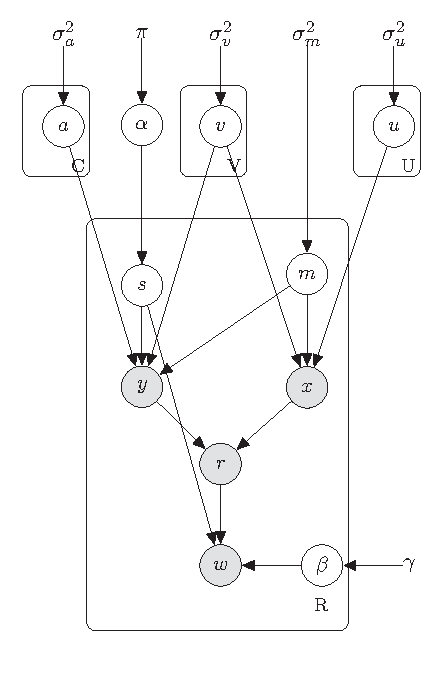
\includegraphics{model.eps}}
\centerline{(a) Plate notation for the CCC model}
\end{minipage}%
\hfill
\vspace{2pt}
\begin{minipage}[b]{.3\linewidth}
\centerline{
\begin{tabular}{|c|}
\hline
Variable \& Interpretation \\\hline\hline
$a(c) \in R^K$ \\ Context aware preference \\\hline
$u \in R^K$ \\ User preference \\\hline
$v \in R^K$ \\ Commodity features \\\hline
$s \in R^C, s_c\in \{0,1\}, \Sigma_c s_c =1$ \\ Context indicators \\\hline
$x \in \{0,1\}$ \\ Context irrelevant rating, partially observable \\\hline
$y \in \{0,1\}$ \\ Context aware rating, partially observable \\\hline
$r \in \{0,1\}$ \\  response observation\\whether the review contains contextual information\\\hline
$\beta \in R^{(C+1)\times |W|}$ \\ Word distribution \\\hline
\end{tabular}}
\vfill
\centerline{(b) List of notations for variables}
\end{minipage}
\caption{The Conditional Contextual Comparison (CCC) Model}
\end{figure}



%???need discussion???
\section{Application}\label{sec:method}
%

 
 
%problem definition
\subsection{ Recommendation}
\subsection{Contextual Information Extraction}


\section{Experiment}\label{sec:exp}
\subsection{Experimental Setup}

\subsection{Context Aware Recommendation}

\subsection{Contextual Phrases Distribution}

\subsection{Parameter Performance}

\subsection{Case Study}

\section{Conclusion}~\label{sec:con}
In this paper, we mainly focus on exploring the potencial of implicit feedback in a review guided context aware recommender system. We present new models, based on the utility surplus theory, to tackle the implicit feedback problem by treating them as complete observations or missing not at random observations. We systematically compare the assumptions and performances of thes models.
The most important academic contribution of this paper is that, to the best of our
knowledge, the unique types of implicit feedback (both context free and context aware) have not yet been studied by the community. Therefore our research might shed some insight into mining online reviews for recommender system, and other applications.
Further research issues include adapting and testfying more assumption in the missing not at random model.
For example, the inter homogenity of online communities, and applying the CPP model to appropriate contexts.
%\section{Acknowledgement}
%Chen Lin is partially supported by China Natural Science Foundation under Grant Nos. NSFC61102136, NSFC61472335, CCF-Tencent Open Research Fund under Grant No. CCF-Tencent20130101, Base Research Project of Shenzhen Bureau of Science,Technology, and Information under Grand No. JCYJ20120618155655087, Baidu Open Research under Grant No.Z153283.
\begin{thebibliography}{10}
\bibitem{Adomavicius2005Incorporating}
Gediminas Adomavicius, Ramesh Sankaranarayanan, Shahana Sen, and Alexander
Tuzhilin.
\newblock Incorporating contextual information in recommender systems using a
multidimensional approach.
\newblock {\em ACM Trans. Inf. Syst.}, 23(1):103--145, January 2005.
\bibitem{Adomavicius2011Context}
Gediminas Adomavicius and Alexander Tuzhilin.
\newblock Context-aware recommender systems.
\newblock In {\em Recommender systems handbook}, pages 217--253. Springer,
2011.
\bibitem{Baltrunas2011Context}
Linas Baltrunas, Bernd Ludwig, Stefan Peer, and Francesco Ricci.
\newblock Context-aware places of interest recommendations for mobile users.
\newblock In {\em Design, User Experience, and Usability. Theory, Methods,
Tools and Practice}, pages 531--540. Springer, 2011.
\bibitem{Baltrunas2009Context}
Linas Baltrunas and Francesco Ricci.
\newblock Context-based splitting of item ratings in collaborative filtering.
\newblock In {\em Proceedings of the Third ACM Conference on Recommender
Systems}, RecSys '09, pages 245--248, New York, NY, USA, 2009. ACM.
\bibitem{Bell2007Scalable}
R.M. Bell and Y.~Koren.
\newblock Scalable collaborative filtering with jointly derived neighborhood
interpolation weights.
\newblock In {\em Data Mining, 2007. ICDM 2007. Seventh IEEE International
Conference on}, pages 43--52. Ieee, 2007.
\bibitem{Biancalana2013Approach}
Claudio Biancalana, Fabio Gasparetti, Alessandro Micarelli, and Giuseppe
Sansonetti.
\newblock An approach to social recommendation for context-aware mobile
services.
\newblock {\em ACM Trans. Intell. Syst. Technol.}, 4(1):10:1--10:31, February
2013.
\bibitem{Bobadilla2013Recommender}
J.~Bobadilla, F.~Ortega, A.~Hernando, and A.~Guti??rrez.
\newblock Recommender systems survey.
\newblock {\em Knowledge-Based Systems}, 46(0):109 -- 132, 2013.
\bibitem{Cai2007MusicSense}
Rui Cai, Chao Zhang, Chong Wang, Lei Zhang, and Wei-Ying Ma.
\newblock Musicsense: Contextual music recommendation using emotional
allocation modeling.
\newblock In {\em Proceedings of the 15th International Conference on
Multimedia}, MULTIMEDIA '07, pages 553--556, New York, NY, USA, 2007. ACM.
\bibitem{Gorgoglione2011Effect}
Michele Gorgoglione, Umberto Panniello, and Alexander Tuzhilin.
\newblock The effect of context-aware recommendations on customer purchasing
behavior and trust.
\newblock In {\em Proceedings of the Fifth ACM Conference on Recommender
Systems}, RecSys '11, pages 85--92, New York, NY, USA, 2011. ACM.
\bibitem{Hariri2012Context}
Negar Hariri, Bamshad Mobasher, and Robin Burke.
\newblock Context-aware music recommendation based on latenttopic sequential
patterns.
\newblock In {\em Proceedings of the Sixth ACM Conference on Recommender
Systems}, RecSys '12, pages 131--138, New York, NY, USA, 2012. ACM.
\bibitem{Hariri2013Query}
Negar Hariri, Bamshad Mobasher, and Robin Burke.
\newblock Query-driven context aware recommendation.
\newblock In {\em Proceedings of the 7th ACM Conference on Recommender
Systems}, RecSys '13, pages 9--16, New York, NY, USA, 2013. ACM.
\bibitem{Heckerman1997Models}
David Heckerman and Christopher Meek.
\newblock Models and selection criteria for regression and classification.
\newblock In {\em Proceedings of the Thirteenth Conference on Uncertainty in
Artificial Intelligence}, UAI'97, pages 223--228, San Francisco, CA, USA,
1997. Morgan Kaufmann Publishers Inc.
\bibitem{Karatzoglou2010Multiverse}
Alexandros Karatzoglou, Xavier Amatriain, Linas Baltrunas, and Nuria Oliver.
\newblock Multiverse recommendation: N-dimensional tensor factorization for
context-aware collaborative filtering.
\newblock In {\em Proceedings of the Fourth ACM Conference on Recommender
Systems}, RecSys '10, pages 79--86, New York, NY, USA, 2010. ACM.
\bibitem{Koren2009Matrix}
Y.~Koren, R.~Bell, and C.~Volinsky.
\newblock Matrix factorization techniques for recommender systems.
\newblock {\em Computer}, 42(8):30--37, 2009.
\bibitem{Levi2012Finding}
Asher Levi, Osnat Mokryn, Christophe Diot, and Nina Taft.
\newblock Finding a needle in a haystack of reviews: Cold start context-based
hotel recommender system.
\newblock In {\em Proceedings of the Sixth ACM Conference on Recommender
Systems}, RecSys '12, pages 115--122, New York, NY, USA, 2012. ACM.
\bibitem{Li2011Towards}
Beibei Li, Anindya Ghose, and Panagiotis~G. Ipeirotis.
\newblock Towards a theory model for product search.
\newblock In {\em Proceedings of the 20th international conference on world
wide web}, pages 327--336, 2011.
\bibitem{Li2010Contextual}
Yize Li, Jiazhong Nie, Yi~Zhang, Bingqing Wang, Baoshi Yan, and Fuliang Weng.
\newblock Contextual recommendation based on text mining.
\newblock In {\em Proceedings of the 23rd International Conference on
Computational Linguistics: Posters}, COLING '10, pages 692--700, Stroudsburg,
PA, USA, 2010. Association for Computational Linguistics.
\bibitem{Liu2005Opinion}
Bing Liu, Minqing Hu, and Junsheng Cheng.
\newblock Opinion observer: Analyzing and comparing opinions on the web.
\newblock In {\em Proceedings of the 14th International Conference on World
Wide Web}, WWW '05, pages 342--351, New York, NY, USA, 2005. ACM.
\bibitem{Liu2013Combining}
Hongyan Liu, Jun He, Tingting Wang, Wenting Song, and Xiaoyang Du.
\newblock Combining user preferences and user opinions for accurate
recommendation.
\newblock {\em Electronic Commerce Research and Applications}, 12(1):14 -- 23,
2013.
\bibitem{Moghaddam2013FLDA}
Samaneh Moghaddam and Martin Ester.
\newblock {The FLDA model for aspect-based opinion mining: addressing the cold
start problem}.
\newblock In {\em Proceedings of the 22nd international conference on World
Wide Web}, pages 909--918. International World Wide Web Conferences Steering
Committee, May 2013.
\bibitem{Ounis2006Terrier}
I.~Ounis, G.~Amati, V.~Plachouras, B.~He, C.~Macdonald, and C.~Lioma.
\newblock {Terrier: A High Performance and Scalable Information Retrieval
Platform}.
\newblock In {\em Proceedings of ACM SIGIR'06 Workshop on Open Source
Information Retrieval (OSIR 2006)}, 2006.
\bibitem{Palmisano2008Using}
C.~Palmisano, A~Tuzhilin, and M.~Gorgoglione.
\newblock Using context to improve predictive modeling of customers in
personalization applications.
\newblock {\em Knowledge and Data Engineering, IEEE Transactions on},
20(11):1535--1549, Nov 2008.
\bibitem{Panniello2009Experimental}
Umberto Panniello, Alexander Tuzhilin, Michele Gorgoglione, Cosimo Palmisano,
and Anto Pedone.
\newblock Experimental comparison of pre- vs. post-filtering approaches in
context-aware recommender systems.
\newblock In {\em Proceedings of the Third ACM Conference on Recommender
Systems}, RecSys '09, pages 265--268, New York, NY, USA, 2009. ACM.
\bibitem{Qu2010Bag}
Lizhen Qu, Georgiana Ifrim, and Gerhard Weikum.
\newblock The bag-of-opinions method for review rating prediction from sparse
text patterns.
\newblock In {\em Proceedings of the 23rd International Conference on
Computational Linguistics}, COLING '10, pages 913--921, Stroudsburg, PA, USA,
2010. Association for Computational Linguistics.
\bibitem{Raghavan2012Review}
Sindhu Raghavan, Suriya Gunasekar, and Joydeep Ghosh.
\newblock Review quality aware collaborative filtering.
\newblock In {\em Proceedings of the Sixth ACM Conference on Recommender
Systems}, RecSys '12, pages 123--130, New York, NY, USA, 2012. ACM.
\bibitem{Rendle2009BPR}
Steffen Rendle, Christoph Freudenthaler, Zeno Gantner, and Lars Schmidt-Thieme.
\newblock Bpr: Bayesian personalized ranking from implicit feedback.
\newblock In {\em Proceedings of the Twenty-Fifth Conference on Uncertainty in
Artificial Intelligence}, UAI '09, pages 452--461, Arlington, Virginia,
United States, 2009. AUAI Press.
\bibitem{salakhutdinov2008probabilistic}
R.~Salakhutdinov and A.~Mnih.
\newblock Probabilistic matrix factorization.
\newblock {\em Advances in neural information processing systems},
20:1257--1264, 2008.
\bibitem{Shi2012CLiMF}
Yue Shi, Alexandros Karatzoglou, Linas Baltrunas, Martha Larson, Nuria Oliver,
and Alan Hanjalic.
\newblock Climf: Learning to maximize reciprocal rank with collaborative
less-is-more filtering.
\newblock In {\em Proceedings of the Sixth ACM Conference on Recommender
Systems}, RecSys '12, pages 139--146, New York, NY, USA, 2012. ACM.
\bibitem{Shi2010Listwise}
Yue Shi, Martha Larson, and Alan Hanjalic.
\newblock List-wise learning to rank with matrix factorization for
collaborative filtering.
\newblock In {\em Proceedings of the fourth ACM conference on Recommender
systems}, RecSys '10, pages 269--272, New York, NY, USA, 2010. ACM.
\bibitem{Si2014Users}
Jianfeng Si, Qing Li, Tieyun Qian, and Xiaotie Deng.
\newblock Users?? interest grouping from online reviews based on topic
frequency and order.
\newblock In {\em World Wide Web}, 17(6):1321?C1342, 2014.
\bibitem{Wang2015CROWN}
S.~Wang, B.~Zou, C.~Li, K.~Zhao, Q.~Liu, and H.~Chen.
\newblock Crown: A context-aware recommender for web news.
\newblock In {\em 2015 IEEE 31st International Conference on Data Engineering},
pages 1420--1423, April 2015.
\bibitem{Marlin2009Collaborative}
Marlin, Benjamin M. and Zemel, Richard S.
\newblock Collaborative Prediction and Ranking with Non-random Missing Data
\newblock In {\em Proceedings of the Third ACM Conference on Recommender Systems}, RecSys '09, pages 5--12, New York, NY, USA, 2009, ACM.
\bibitem{Wojnicki2008Word}
\newblock A.C. Wojnicki, D. Godes.
\newblock Word-of-Mouth as Self-Enhancement
\newblock In {\em HBS Marketing Research Paper No.
06-01}, 2008.
\bibitem{samuelson1937note}
\newblock Paul A Samuelson
\newblock A note on measurement of utility
\newblock In {\em The Review of Economic Studies}, pages 155--161, 4(2), 1937
\bibitem{Marcelo2016Mining}
\newblock Marcelo G. Manzato , Marcos A. Domingues , Arthur C. Fortes , Camila V. Sundermann , Rafael M. D'addio , Merley S. Conrado , Solange O. Rezende , Maria G. Pimentel.
\newblock Mining unstructured content for recommender systems: an ensemble approach,
\newblock In {\em Information Retrieval} 19(4), p.378-415, August 2016

\end{thebibliography}
\end{document}